\documentclass[landscape]{article}
\usepackage[a4paper,margin=3mm,landscape]{geometry}
\usepackage[scaled=0.92]{helvet}
\usepackage{multicol, multirow}
\usepackage{makecell}
\usepackage{array} 
\usepackage[table]{xcolor}
\usepackage{enumitem} 
\usepackage{amssymb}
\usepackage{graphicx}
\setlist{nosep}

\graphicspath{{./images/}}

\pdfinfo{
    /Title (CS3219 Cheatsheet.pdf)
    /Creator (TeX)
    /Producer (pdfTeX 1.40.0)
    /Author (Selwyn Ang)
    /Subject (CS3219)
    /Keywords (CS3219, Cheatsheet, NUS, Software Engineering Principles and Patterns) 
}

% Turn off header and footer
\pagestyle{empty}


\makeatletter
\DeclareRobustCommand\smaller{\@setfontsize\smaller{6pt}{6.5pt}}
\makeatother

% redefine section commands to use less space
\makeatletter
\renewcommand{\section}{\@startsection{section}{1}{0mm}%
  {-0.1ex plus -0.1ex minus -0.1ex}%
  {0.1ex plus .1ex minus 0.1ex}%
{\normalfont\small\bfseries}}
\renewcommand{\subsection}{\@startsection{subsection}{2}{0mm}%
  {-0.1ex plus -0.1ex minus -0.1ex}%
  {0.1ex plus .1ex minus 0.1ex}%
{\normalfont\scriptsize\bfseries}}
\renewcommand{\subsubsection}{\@startsection{subsubsection}{3}{0mm}%
  {-0.1ex plus -0.1ex minus -0.1ex}%
  {0.1ex plus .1ex minus 0.1ex}%
{\normalfont\smaller\bfseries}}%
\makeatother



\renewcommand{\familydefault}{\sfdefault}
\renewcommand\rmdefault{\sfdefault}
%  makes nested numbering (e.g. 1.1.1, 1.1.2, etc)
\renewcommand{\labelenumii}{\theenumii}
\renewcommand{\theenumii}{\theenumi.\arabic{enumii}.}
\renewcommand\labelitemii{•}
\renewcommand\labelitemiii{•}

\setlength{\parindent}{0pt}
\setlength{\parskip}{0pt plus 0.5ex}
\setlength{\columnsep}{0.2cm}
%% adjust spacing for all itemize/enumerate
\setlength{\leftmargini}{0.5cm}
\setlength{\leftmarginii}{0.5cm}
\setlist[itemize,1]{leftmargin=2mm,labelindent=1mm,labelsep=1mm}
\setlist[itemize,2]{leftmargin=2mm,labelindent=1mm,labelsep=1mm}
\setlist[itemize,3]{leftmargin=2mm,labelindent=1mm,labelsep=1mm}
\setlist[enumerate,1]{leftmargin=2mm,labelindent=1mm,labelsep=1mm}
\setlist[enumerate,2]{leftmargin=2mm,labelindent=1mm,labelsep=1mm}
\setlist[enumerate,3]{leftmargin=2mm,labelindent=1mm,labelsep=1mm}

% tightcenter
\newenvironment{tightcenter}{%
  \setlength\topsep{0pt}
  \setlength\parskip{0pt}
  \begin{center}
    }{%
  \end{center}
}

% boxed
\newenvironment{tightbox}{%
  \setlength\topsep{0pt}
  \setlength\parskip{0pt}
  \begin{center}
    \begin{tabular}{|@{\hspace{\dimexpr\fboxsep+0.5\arrayrulewidth}}c@{\hspace{\dimexpr\fboxsep+0.5\arrayrulewidth}}|}
      \hline
    }
    {%
    \\ \hline
    \end{tabular}
  \end{center}
}

% fixed width box
\newenvironment{fixedbox}[1][0.7]{
  \setlength\topsep{0pt}
  \setlength\parskip{0pt}
  \begin{center}
    \begin{tabular}{|>{\centering\arraybackslash}m{#1\linewidth}|}
    \hline
  }{
  \\ \hline
  \end{tabular}
  \end{center}
}

% definition of a new term
\usepackage{soul}
\definecolor{paleyellow}{RGB}{251,243,218}
\newcommand{\definition}[2][]{\sethlcolor{paleyellow}\hl{\textbf{#2}} #1  $\rightarrow$}
% inline definition
\newcommand{\ildefinition}[1]{\sethlcolor{paleyellow}\hl{\textbf{#1}}}

% important note (attention)
\newcommand{\attention}{{\color{red}\textbf{! }}}

% nice proof
\newenvironment{niceproof}[1][Proof]
{%
  \sbox0{\textit{#1}. }%
  \list{}{\labelwidth\wd0 \leftmargin\wd0 \labelsep 0pt }
\item[\usebox0]}
  {\endlist}


\usepackage{color, soul}
\usepackage{listings}
\usepackage{inconsolata}

\definecolor{codegreen}{rgb}{0,0.6,0}
\definecolor{codegray}{rgb}{0.5,0.5,0.5}
\definecolor{codepurple}{HTML}{C42043}
\definecolor{backcolour}{HTML}{F2F2F2}
\definecolor{bookColor}{cmyk}{0,0,0,0.90}

\newcommand{\code}[1]{\texttt{\sethlcolor{backcolour}\hl{$\,$#1$\,$}}}

% SQL code blocks
% define SQL styles
\lstdefinestyle{mySQL}{%
  language=SQL,
  backgroundcolor=\color{backcolour},
  commentstyle=\color{codegreen},
  keywordstyle=\color{codepurple},
  numberstyle=\numberstyle,
  stringstyle=\color{codepurple},
  basicstyle=\scriptsize\ttfamily,
  breaklines=true,
}



% --------------------------------------------------------

\begin{document}
\raggedright
\tiny
\begin{multicols*}{5}
    \setlength{\columnseprule}{0.25pt}

    \begin{tightcenter}
        \fbox{%
          \parbox{0.8\linewidth}{\centering \textcolor{black}{
              {\Large\textbf{CS3219}}
            \\ \normalsize{AY24/25 SEM 1}}
            \\ {\footnotesize \textcolor{gray}{github/SelwynAng}}
          }%
        }
    \end{tightcenter}
    
    \section{Software Applications, Deployment \& Development Processes}
    \subsection{Cloud Computing}
    \begin{itemize}
      \item Software infrastructure hosted on an external data center with services delivered over the internet
      \item \underline{Different models}
      \begin{enumerate}
        \item \textbf{On-site:} User manages applications, data, runtime, middleware, OS, virtualisation, servers, storage, networking
        \item \textbf{IaaS:} User manages applications, data, runtime, middleware, OS $|$ service provider manages the rest
        \item \textbf{PaaS:} User manages applications, data $|$ service provider manages the rest
        \item \textbf{SasS:} Service provider manages everything
      \end{enumerate}
      \item Cloud native is the software approach of building, deploying and managing modern applications in cloud computing environments
    \end{itemize}

    \subsection{Deployment (Software Delivery)}
    \begin{itemize}
      \item Deployment comprises activities that make the software available for use after development (process between software acquisition and execution)
      \item \textbf{Deployment Issues:} Integration of the internet and related advances (Portability), Large-scale content delivery (Availability, Performance), Heterogeneous platforms (Interoperability), Dependency and change management (Maintainability), Coordination and communication among components (Performance), Security
      \item \textbf{Deployment Mechanisms:}
      \begin{enumerate}
        \item \underline{Bare metal:} (+): Complete control, physical isolation $|$ (-): Wasted hardware resources, cost, scalability issues
        \item \underline{Virtual machine:} (+): Improved resource utilization, flexible, scalable $|$ (-): Vulnerable to side-channel attacks, noisy neighbor problem
        \item \underline{Container:} (+): Lighter than VM, write once run anywhere, granular control $|$ (-): Not suitable for all apps, not suitable for performance-critical applications
      \end{enumerate}
      \item \textbf{Container VS Orchestrator VS Serverless:}
      \begin{itemize}
        \item \underline{Container:} Provide the platform for building \& distributing services
        \item \underline{Orchestrator:} Separate software that integrate \& coordinate many parts, scale up/down deployment, provide fault tolerance, provide communication among containers
        \item \underline{Serverless:} Cloud provider dynamically manages the allocation and provisioning of servers (used for small, stateless, event-driven workloads, e.g., processing an image upload, API endpoints)
      \end{itemize}
    \end{itemize}

    \subsection{Software Development Process:}
    \begin{itemize}
      \item Use waterfall model when requirements are well-understood, fixed, and effort predictable $|$ Use iterative development for fuzzy and evolving requirements
      \item \textbf{CI/CD Pipeline:}
      \begin{itemize}
        \item \underline{Continuous Integration:} Development practice that requires developers to integrate code into shared repo several times a day $\rightarrow$ Each check-in is then verified via automated build
        \item \underline{Continuous Delivery:} Ensuring that every good build is potentially ready for production release (Manual deployment to production)
        \item \underline{Continuous Deployment:} Automating release of a good build to production environment (Auto deployment to production)
      \end{itemize}
      \item \textbf{DevOps:} Blends software development \& operations staff and tools $\rightarrow$ Reduce time between committing change to system and the change being placed into production while ensuring high quality
    \end{itemize}

    \section{Specifying Software Requirements}
    \subsection{Requirements}
    \begin{itemize}
      \item \textbf{Definition:} Capability needed by a user, Capability that must be met or possessed by a system, Documented representation of a condition or capability, Specification what should be implemented
      \item \textbf{User centric Requirement:} Eg. As a user, I can upload a 20 mb image file into the system so that I can retain the original image without loss of quality
      \item \textbf{Product centric Requirement:} Eg. The system will support a range of graphic file formats up to 20 mb in size
      \item \textbf{Requirement Development Phases:} Elicitation $\rightarrow$ Analysis $\rightarrow$ Specification $\rightarrow$ Validation
      \item \textbf{Outcomes of Requirements Development Process:} (1): Software Requirements Specification (SRS), (2): Rights, responsibilities \& agreements
      \item \textbf{SRS VS Product Backlog:} Product Backlog (Repo of work to be done, facilitates prioritization of work \& planning), SRS (in-depth description of software product to be developed, direct/indirect requirements of system, only tells what work is to be done)
      \item \textbf{Validation:} Whether you have written the right requirements
      \item \textbf{Verification:} Whether you have written the requirements right
    \end{itemize}

    \subsection{Types of Requirements}
    \begin{enumerate}
      \item \textbf{Business:} Describe why organization is implementing the system
      \item \textbf{User:} Describe goals or tasks user must be able to perform with the product
      \item \textbf{System:} Describes connections between your system and outside world
      \item \textbf{Functional:} Specifies something the system should do
      \item \textbf{Non-functional/Quality:} Describes something not directly related to system functionality, but how well the system works
      \item \textbf{Constraints:} States a limitation on design or implementation choices
      \item \textbf{Data}
    \end{enumerate}
    NOTE: Business Req to be in Vision and Scope document, User Req to be in User Requirements document, FRs, NFRs, System Req, Constraints to be in SRS

    \subsection{Software Quality Attributes:}
    \begin{itemize}
      \item \textbf{External:} Observed when software is executing, impacts UX, develops user's perception of software quality \textit{(Eg. Availability, Performance, Robustness, Safety, Security, Reliability, Integrity, Deployability, Compatibility, Installability, Usability, Interoperability)}
      \begin{enumerate}
        \item \underline{Security:} Specifying security features at SRS ensures that acceptance tests include testing for security $|$ About privacy, authentication, integrity
        \item \underline{Safety:} About whether a system can harm someone or something
        \item \underline{Performance:} Responsiveness of system, impacts UX, includes response time, throughput, data capacity, dynamic capacity, predictability in real-time systems, latency, behavior in degraded modes or overloaded conditions
        \item \underline{Availability:} Planned uptime of system ($\frac{Uptime}{Uptime + Downtime}$)
        \item \underline{Usability:} Measures the effort required to prepare input, operate, and decipher output of software
      \end{enumerate}
      \item \textbf{Internal:} Not directly observed when software is executing, perceived by developers/maintainers, encompasses aspects of design that may impact external attributes \textit{(Eg. Efficiency, Scalability, Verifiability, Portability, Maintainability, Testability, Modifiability, Reusability)}
      \begin{enumerate}
        \item \underline{Scalability:} Ability of application to accommodate growth in application usage (\textit{Vertical scaling:} increasing capacity of system by adding capability to machines used which is easier to maintain, but causes single point of failure $|$ \textit{Horizontal Scaling:} increasing capacity of system by adding additional machines which increases fault tolerance, but adds costs and complexity)
      \end{enumerate}
    \end{itemize}

    \section{High Level Design - Software Architecture}
    \subsection{Software Architecture}
    \begin{itemize}
      \item \textbf{Definition:} Structure of system, which comprise software components, externally visible properties of those components, and the relationships among them
      \item \textbf{Consists of:} (1): \underline{Component} (element that models an application-specific function, responsibility, requirement, task, process), (2): \underline{Configuration} (Topology/Structure), (3): \underline{Connector} (Element that models interactions among components for purpose of transfer of control/data)
    \end{itemize}

    \subsection{Common Definitions}
    \begin{enumerate}
      \item \textbf{Control Flow:} Reasoning is on computation order, how the focus of control moves throughout the execution
      \item \textbf{Data Flow:} Reasoning is on data availability, transformation, latency, how data moves through collection of computations
      \item \textbf{Call and Return:} Control moves from 1 component to another and back, can be hierarchical/non-hierarchical
      \item \textbf{Message:} Data sent to a specific address (each component has a unique address other components can send messages to)
      \item \textbf{Event:} Data emitted from a component for anyone listening to consume (message sent to publishing infrastructure where consumers may later retrieve, is immutable, ordered in sequence of creation)
    \end{enumerate}

    \subsection{Decomposition \& Packaging}
    \begin{itemize}
      \item \textbf{Slicing:} (1): \underline{Horizontal Slicing:} designing by layers, (2): \underline{Vertical Slicing:} designing by feature
      \item \textbf{Principle of Modularity:} Modularization results in shorter development time, better flexibility, better comprehensibility $|$ Decomposing big chunk into smaller chunks with well-defined APIs
      \item \textbf{Types of Cohesion:} Functional, Layer, Communicational, Sequential, Procedural, Temporal, Utility
      \item \textbf{Types of Coupling:} Content, Global variables, Control, Data, External, Temporal, Inclusion/import
    \end{itemize}

    \subsection{Architectural Styles}
    \begin{itemize}
      \item \textbf{How code is divided:}
      \begin{enumerate}
        \item \underline{Technical Partitioning:} Focus on separation of concerns (Eg. Presentation, Services, Persistence)
        \item \underline{Domain Partitioning:} Aligned with the domain (Eg. Customer, Shipping, Payment)
      \end{enumerate}
      \item \textbf{How is it deployed:}
      \begin{enumerate}
        \item \underline{Monolithic:} Deploy all logical components that make up the application as 1 unit, application runs as 1 process
        \item \underline{Distributed:} Application consists of independent logical components, logical components run as individual processes, communicate over network
      \end{enumerate}
      \item \textbf{Types:}
      \begin{enumerate}
        \item \underline{Layered (Technical \& Monolith):}
        \begin{itemize}
          \item Lower level layers provides functionality for higher level layers
          \item \textit{Open layer architecture:} 1 layer can talk to another layer, which can be layers away
          \item \textit{Close layer architecture:} 1 layer can only talk to a neighboring layer
          \item More layers result in scalability by allowing each layer to run in different server, but communication becomes expensive
          \item Less layers result in performance optimization, no context-switching overheads, but difficult to modify, impractical
        \end{itemize} 
        \item \underline{Modular Monolith (Domain \& Monolith):} Separation by domain (business) concern, reduces coupling (Eg. Order domain, recipe domain, where each domain consists of presentation, logic \& persistence layers)
        \item \underline{Event-driven (Technical \& Distributed):}
        \item \underline{Microservices (Domain \& Distributed):}
        \item \underline{Pipe \& Filter:}
        \begin{itemize}
          \item Data enters system and flows through components one at a time until data is assigned to some final destination (Data Sink)
          \item Components consist of \textit{Filters, Data Source, Data Sink}, where each component can read and produce
          \item \textit{Filter} transforms input streams, computes incrementally $\rightarrow$ output begins before input is consumed, is independent, shares no state with other filters
          \item \textit{Pipe} transmits output of 1 filter to input of another filter
          \item \textit{Purpose:} Divides the app's task into several self-contained data process steps \& connect these steps to data processing pipeline via intermediate data buffers $\rightarrow$ Data flows in streams (good for image, audio, video, or batch data processing with limited user interaction)
          \item We can use files as pipes that capture output of one process and feed input to another process
        \end{itemize}
        \item \underline{Model-View-Controller}
        \begin{itemize}
          \item View (widgets in UI, buttons, text boxes), Controller (coordinates btw. Model and View), Model (business logic)
          \item \textit{Benefits:} Separation of concerns, Facilitates extensibility, Restricted communication reduces complexity \& side effects, Better testability (easy to mock components), Frameworks provide MVC solution
          \item \textit{Web MVC:} Controller (handles HTTP requests, select model, prepare view), View (renders HTTP response), Model (logic \& persistence)
          \item \textit{Single Page Applications (SPA):} Send query and retrieve data in background without refreshing webpage
        \end{itemize}
      \end{enumerate}
    \end{itemize}

    \subsection{REST Architecture} (Not an architecture by itself)
    \begin{itemize}
      \item \textbf{Definition:} Defines constraints for transferring, accessing, and manipulating textual data representations in a stateless manner across a network of systems $\rightarrow$ Provide uniform interoperability between different applications on the internet (HTTP to request access and use data)
      \item \textbf{Constraints:}
      \begin{enumerate}
        \item \underline{Client-Server:} REST apps should have client-server architecture for separation of concerns $\rightarrow$ Improve portability of UI \& scalability of server components
        \item \underline{Stateless:} No client state (session) maintained on server $\rightarrow$ Server is bound by no. of concurrent requests \& not the no. of clients interacting $\rightarrow$ Improve scalability, reliability, monitoring
        \item \underline{Cache-able:} Response from server should include if data is cache-able or not $\rightarrow$ Client returns data from its cache in response to subsequent requests $\rightarrow$ Improves network efficiency, but client can potentially receive stale data
        \item \underline{Layered System:} App must be organized as a layered system $\rightarrow$ Improved overall system complexity by restricting complexity to individual layers, intermediary servers may improve system availability \& performance, provide data transformation \& filtering 
        \item \underline{Uniform Interface:} Uniform way of interacting with a given server irrespective of device/application, exploits HTTP/HTTPS requests \& responses
        \begin{itemize}
          \item \textit{Resource Identifier:} Global, unique method to identify resources
          \item \textit{Resource Representation:} Components perform operations on resource representations
        \end{itemize}
        \item \underline{Code-on-demand:} Allow client functionality to be extended by downloading executable code, simplifies client from having to pre-implement all functionality, allows extensibility
      \end{enumerate}
      \item \textbf{Advantages of REST:} Systems are less tightly coupled, provides scalability, usability, accessibility
      \item \textbf{Disadvantages of REST:} Being stateless decrease network performance by increasing repetitive data sent in series of queries $|$  Using URI degrade efficiency since info is transferred in standardized form rather than one which is specific to app's needs
    \end{itemize}

    \section{Microservices Architecture}
    \subsection{Microservices Architectural Style}
    \begin{enumerate}
      \item A single application as a suite of small services
      \item Each microservice offers a well-defined business capability (Features in microservice should be highly related)
      \item Each microservice is defined to be developed \& deployed independently (Services do not need to share any of their code or implementation with other services $\rightarrow$ minimal dependency on each other, services are owned by different teams)
      \item Microservices communicate with each other through well-defined mechanisms (Synchronous: RESTful APIs, gRPC, GraphQL, Asynchronous: Event-based publish \& subscribe)
    \end{enumerate}
    
    \subsection{Domain Driven Design}
    \begin{itemize}
      \item Complex system is fundamentally a collection of multiple domain models (sub-domains)
      \item\textbf{Domain:} Problem space that a business occupies and provides solution to
      \item \textbf{Sub-domain:} Component of main domain, belongs to problem space
      \item \textbf{Bounded Context:} High cohesive boundary relevant to the sub-domain $\rightarrow$ Belongs to solution space $\rightarrow$ Not the same as Microservice (BC is a concept, while MS is an implementation $\rightarrow$ Ideally, a MS should align with a BC \& it is possible for a BC to map to multiple MSes \& a MS to implement multiple BCs)
      \item \textbf{Types of Collaborations between different Bounded Contexts (BC):}
      \begin{enumerate}
        \item \underline{Shared Kernel:} 2 contexts are developed independently, but they end up overlapping some subset of each other's domain
        \item \underline{Upstream-Downstream:} 2 contexts are in provider (upstream) - consumer (downstream) relationship
        \begin{itemize}
          \item \textit{Supplier-Customer Relationship:} Supplier is the BC that provides a service, functionality or data to another BC, while Customer is the BC that consumes the functionality/data (Eg. Order Context supplies order data, Recommendation Context fetches the order data)
          \item \textit{Conformist Relationship:} 1 BC (the conformist) fully adopts the model of another BC without trying to impose its own requirements or interpretations (Eg. Payment service must align entirely with the bank's API and data structures, regardless of whether it fits the payment service's internal domain model or not)
        \end{itemize}
      \end{enumerate}
      \item \textbf{Aggregate:} A cluster of related objects that we treat as a single unit for purpose of data changes (Has \textit{transactional boundary}, which means any changes to aggregate will either all succeed or none will succeed $|$ Has \textit{consistency boundary}, which means all processes or objects external to aggregate are only allowed to read aggregate's state \& its state can only be modified by executing corresponding methods of aggregate's public interface)
      \item \textbf{Aggregate Root:} Parent entity of the aggregate $\rightarrow$ designated as aggregate's public interface
    \end{itemize}

    \subsection{Event Storming}
    \begin{itemize}
      \item \underline{Command} causes \underline{Events} (Eg. User/external system issues a command)
      \item We treat \underline{Aggregate} as a unit for the purpose data changes $\rightarrow$ Eg. Order Processing Aggregate consists of Confirm order Command \& Order confirmed Event
      \item \underline{Policy:} WHEN event THEN command (basically links 2 aggregates together, Eg. When payment card is submitted event happens, then execute confirm order command)
      \item A BC solves 1 problem \& can contain more than 1 aggregate
      \item 2 different aggregates can be created to solve 1 problem delimited by 1 BC
    \end{itemize}
    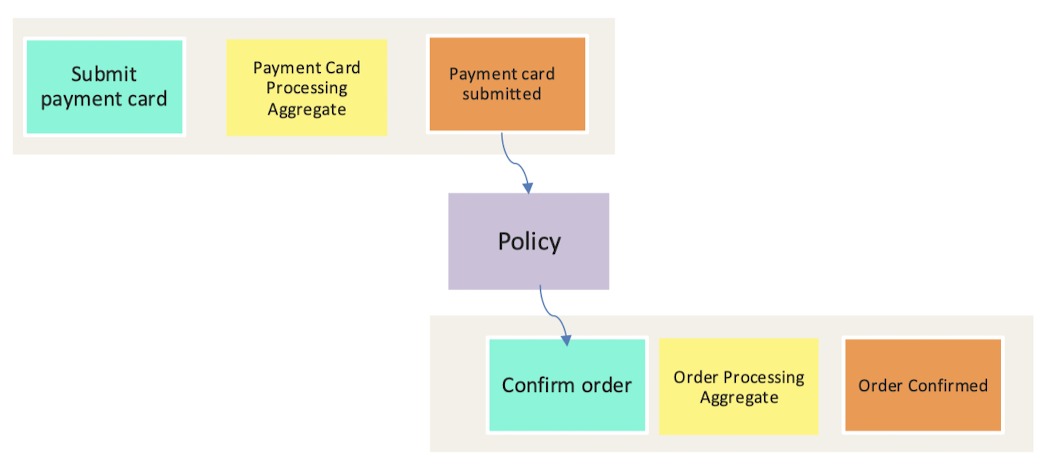
\includegraphics[width=0.75\linewidth]{2_event_storming.png}

    \section{Data Patterns in Microservice Architecture}
    \subsection{Database-server-per-service Pattern}
    \begin{itemize}
      \item Each service has its own database server
      \item (+): Loose coupling, allow scaling services at database level, easier to replace underlying database technology to something appropriate with each service
      \item (-): Hundreds of microservices $\rightarrow$ Different kinds of database $\rightarrow$ Explosion of no. of DB clusters $\rightarrow$ Expensive, unmanageable
      \item However, Data independence $\neq$ Each microservice to own cluster of DB  $\rightarrow$ Microservices do not modify the same data by having:
      \begin{enumerate}
        \item \underline{Private-tables-per-service:} Each service owns a set of tables that must only be accessed by that service
        \item \underline{Schema-per-service:} Each service has a database schema that is private to that service
      \end{enumerate}
    \end{itemize}

    \subsection{Data Delegate Pattern}
    \begin{itemize}
      \item Multiple services require data from a single table $\rightarrow$ Not loosely coupled
      \item Can be solved via Data Delegate Pattern (hide shared data behind a delegate service) $\rightarrow$ Authoritative service for all things related to the other services which require common data $\rightarrow$ Stop accessing database directly from other services
    \end{itemize}

    \subsection{Data Lake Pattern}
    \begin{itemize}
      \item Data lake is a read-only, query-able data sink (shared space containing copy of data from all concerned microservices) $\rightarrow$ Owner microservices just stream relevant data into data lake
    \end{itemize}

    \subsection{Sagas Pattern}
    \begin{itemize}
      \item Every step of a transaction defines a compensating action $\rightarrow$ Compensating action executes if we need to roll back the transaction due to later failure $\rightarrow$ Compensating action is registered on a routing slip \& passed along to next step $\rightarrow$ If 1 of the later steps fails, it kicks off execution of all compensating actions on routing slip, "undo" modifications \& bring system to reasonably compensated state 
      \item Sagas $\neq$ ACID transactions $\rightarrow$ Sagas does not promise that when a distributed transaction is rolled back, system will necessarily get back to initial state (Eg. Initial state has 0 notifications, but if we cancel reservation, final state has 2 notifications)
      \item Sequence of events does matter \& should be constructed carefully $\rightarrow$ Better to move steps that are harder to compensate for towards end of transaction (Eg. Move notification to end of process, would save from having to send a lot of correction messages)
    \end{itemize}

    \subsection{Event Sourcing}
    \begin{itemize}
      \item \textbf{Definition:} Is about storing facts and any time you have state change $\rightarrow$ For each modification of state, log (store) the event representing the result of the action (Instead of focusing on persisting the state of the app, you should persist the stream of events which got it into its current state)
      \item \textbf{Event:} Source of truth, \textbf{System State:} Series of consecutive events
      \item \textbf{Event Sourcing VS Relational Modelling:}
      \begin{itemize}
        \item \underline{Relational Modelling:} Store a state of something (Eg. Current price of economy seat on a flight)
        \item \underline{Event Sourcing:} Store facts, incremental changes of the data $\rightarrow$ Current state of system is a derivative, a value that is calculated from the events
      \end{itemize}
      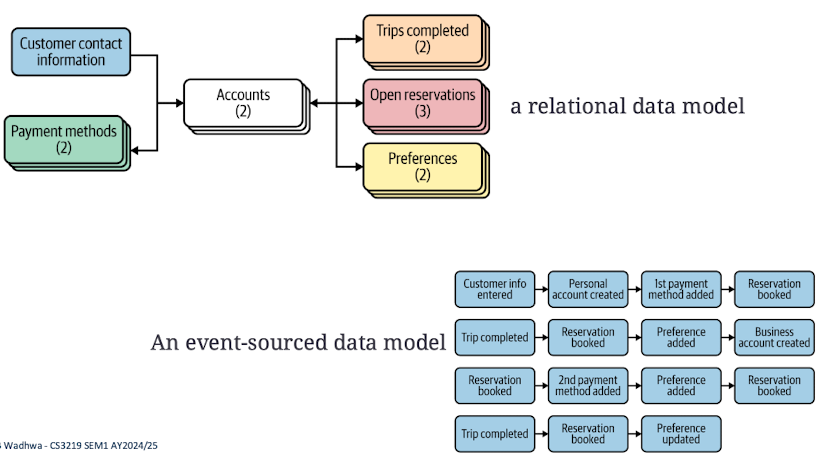
\includegraphics[width=0.85\linewidth]{3_event_sourcing_vs_relational_modelling.png}
      \item \textbf{Event:} 
      \begin{itemize}
        \item Has 3 parts (unique id, event type, data)
        \item Events acts as data that describes some action/fact, Events are notifications of some change in state/data, Events are recordings of what happened
        \item \underline{Projection} function takes current state and a new event to calculate new state $\rightarrow$ Take rolling snapshots (saving projections) to speed up calculation of new state from the last snapshot
      \end{itemize}
      \item \textbf{Event Store:} Database storage that can reliably store a sequence of data entries (Store new events, assign correct sequence, notify event subscribers)
    \end{itemize}

    \subsection{Command Query Responsibility Segregation (CQRS)}
    \begin{itemize}
      \item The way we query \& the way we store data do not have to be the same $\rightarrow$ Separate write path from read path (Should something go wrong, internal state of database can be recovered from the log \& writes and reads can be optimized independently)
      \item \textbf{Commands:} Operations that change application state \& return no data (have side effects within application)
      \item \textbf{Queries:} Operations that return data but do not change application state 
      \item Model used for commands will differ from model used for queries (Data can be stored in different tables/databases for command and query models)
    \end{itemize}

    \section{More Patterns in Microservices Architecture}
    \subsection{Service Instance per Host Pattern}
    \begin{itemize}
      \item Run each service instance in isolation on its own host
      \item \textbf{Service Instance per VM:} Package each service as a VM image $\rightarrow$ Each service instance is a VM
      \item \textbf{Service Instance per Container:} Each service instance runs in its own container $\rightarrow$ Container image is a file system image consisting of the applications \& libraries required to run the service
    \end{itemize}

    \subsection{Immutable Infrastructure \& Infrastructure as Code}
    \begin{itemize}
      \item \textbf{Immutable Infrastructure:} Cannot be changed after it is created (updating immutable object requires it to be destroyed and replaced with a new one) $\rightarrow$ Contain behavior and structures that are easier to predict \& reproduce because they do not change
      \item \textbf{Infrastructure as Code:} All infrastructure must be represented as a set of machine-readable files/code $\rightarrow$ Config files to specify cloud resources needed for deployment $\rightarrow$ Benefits include speed (no humans needed for deployment), consistency (avoid human errors), accountability (traceable via code)
    \end{itemize}
    
    \subsection{Service Collaboration \& Communication}
    \begin{itemize}
      \item \textbf{Service Collaboration:}
      \begin{enumerate}
        \item \underline{Orchestration:} Rely on central brain to guide and drive process (Eg. Service A sends instructions to other services directly)
        \item \underline{Choreography:} Inform each part of system of its job, let them work out the details (Eg. Service A publishes an event that other services subscribe to)
      \end{enumerate} 
      \item \textbf{Service Communication:}
      \begin{enumerate}
        \item \underline{Request/Sync Response:} Client makes a request to service \& waits for a response
        \item \underline{Notification:} Client sends a request to service but no reply is expected or sent (one-way request)
        \item \underline{Request/Async Response:} Client sends a request to service, which replies asynchronously
      \end{enumerate}
    \end{itemize}

    \subsection{Event Driven VS Request-Response Communication}
    \begin{itemize}
      \item \textbf{Event-Driven:} Async pattern, Real-time data, Loose coupling between components in the system (No service knows of existence of any other service, and no service owns the entire workflow), Event (something happened), Best for cases where components need to react to changes in state/real-time data processing is needed (Eg. IoT systems, real-time analytics)
      \item \textbf{Request-Response:} Sync pattern, Introduces latency (if requester waits for response), Tighter coupling since requester needs to know details of responder, Request (do this), Best for cases where client needs specific info (Eg. web APIs, database queries)
      \item \underline{Real-time data:} Data that is published as it is generated, with no known end of data being published $\rightarrow$ Travelling in streams/queues that are built to handle large volumes of data
    \end{itemize}

    \subsection{API Gateway}
    \begin{itemize}
      \item A server that is the single point of entry into the system
      \item Encapsulates internal system architecture \& provides an API that is tailored to each client
      \item Have other responsibilities such as authentication, monitoring, load balancing, caching, etc
      \item \textbf{Backends for Frontends:} A dedicated backend service is created for each frontend interface (e.g., web, mobile, or other client applications) $\rightarrow$ Allows each frontend to interact with its own backend service, which is tailored to its specific needs
    \end{itemize}

    \subsection{Service Discovery}
    \begin{itemize}
      \item \textbf{Service Discovery:} API Gateway needs to know location (IP address and port) of each microservice with which it communicates
      \begin{enumerate}
        \item \underline{Client-side Discovery Pattern:} Client queries a service registry \& determines network locations of available service instances $\rightarrow$ then uses a load-balancing algorithm to select 1 of the available service instances \& makes a request
        \item \underline{Server-side Discovery Pattern:} Client makes a request to service via load balancer $\rightarrow$ Load balancer queries service registry \& routes each request to an available service instance
        \item \underline{Service Registry Pattern:} Service instances are registered with service registry (database of services, their instances \& their locations) on startup \& deregistered on shutdown $\rightarrow$ Client of the service and/or routers query the service registry to find available instances of a service
      \end{enumerate}
    \end{itemize}

    \section{Event Driven Architecture}
    \subsection{Events}
    \begin{itemize}
      \item \textbf{Definition of Event:} Way for a software component to let rest of system know that something important has just happened (allow passing of info between components)
      \item \textbf{Initiating Event:} Originates from an end user \& kicks off a business process
      \item \textbf{Derived Event:} Internal events generated in response to initiating event
      \item \textbf{Structure of Event:}
      \begin{itemize}
        \item Events are typically represented in key/value format (Key: For ID, routing and aggregation operations on events $|$ Value: Complete details of event)
        \item \underline{Unkeyed:} Describes a singular statement of fact (Eg. typically used for system-wide notifications or triggers that are consumed by subscribers interested in general behaviors rather than specific entities) $|$ \underline{Entity:} Unique thing and is keyed on the unique ID of that thing $|$ \underline{Keyed:} Contains a key but does not represent entity
      \end{itemize}
    \end{itemize}

    \subsection{Asynchronous Communication}
    \begin{itemize}
      \item \textbf{Definition:} When software component broadcasts info to other components, it does not wait for response, nor does it care if other components are available or not (Fire-and-forget)
      \item \textbf{Diagram notation:} Dotted lines for async, Solid lines for sync
      \item \textbf{Pros (+):} Better responsiveness (less time to get response for a request), Better availability (other components' availability don't matter)
      \item \textbf{Cons (-):} More complex/fragmented error-handling than sync comms 
    \end{itemize}

    \subsection{Event Driven Architecture (EDA)}
    \begin{itemize}
      \item \textbf{Definition:} Way of designing \& building apps that are based on exchange of events (relies on async comms when sending \& receiving events)
      \item \textbf{Components in EDA:} (1): \underline{Event Producers (Publishers):} Publish data into streams/queues $|$ \underline{Event Brokers:} Implements an event broker/event bus $|$ \underline{Event Consumers (Subscribers):} Listen for \& consume event data
      \item \textbf{EDA VS Microservices (MS) Architecture:}
      \begin{enumerate}
        \item \underline{Communication \& Performance:} EDA relies on async comms (fast), MS communicates via sync using REST and occasionally async comms (sync comms creates latency)
        \item \underline{Bounded Contexts \& Data Ownership:} Nice-to-have for EDA, Foundational for MS
        \item \underline{Event VS Request}: EDA is built on event processing (responding to something that has happened), MS is built on request processing (responding to something that needs to happen)
      \end{enumerate}
    \end{itemize}

    \subsection{Event Driven Microservices}
    \begin{itemize}
      \item \textbf{Definition:} Microservices communicate by producing \& consuming events (Each event stream has 1 and only 1 producing MS $\rightarrow$ This MS is the owner of each event produced to that stream)
      \item \textbf{Event Data:} Serves as data storage \& communication mechanism between services
      \item \textbf{Event Broker:} 
      \begin{itemize}
        \item Receives events, holds/stores events, and provides events for consumption
        \item Event brokers use immutable, append-only event log $\rightarrow$ Preserves state of event ordering, where events are given auto incrementing index ID
        \item Consumer service "seeks" to index ID of last message it read (offset), then scans sequentially, and reads messages in order while recording its new index ID in the partition
        \item \underline{Traits of Event Broker:} Immutability (can alter previous data only by publishing new event with updated data), Ordering (data is served to consumers in same order it was published), Indexing (events are assigned indexes), Partitioning (event streams are partitioned into sub-streams), Infinite retention (Events can be retained for infinite time), Replayability (Any consumer can read whatever data it requires)
        \item \underline{Event Partitions:} Producers write events over many partitions, each partition is an append-only event log, load-balanced consumers share the partitions between them
        \item \underline{Scalability:} Reading \& writing can be done in parallel with events in partitions $\rightarrow$ Scaling is straightforward (with Kafka, hitting scalability wall is impossible)
      \end{itemize}
    \end{itemize}

    \section{Scalability}
    \subsection{Goal of Scalability}
    \begin{itemize}
      \item Increase capacity in some app-specific dimension by:
      \begin{enumerate}
        \item Increase \# of requests that a system can process in a given time period
        \item Increase amount of data to process \& manage
        \item Increase resources (CPU, memory, servers)
      \end{enumerate}
      \item \textbf{2 strategies to scale:}
      \begin{enumerate}
        \item Replicate software processing resources (eg. sever) to provide more capacity to handle requests \& thus increase throughput
        \item Optimize available resources by using more efficient algorithms, adding extra indexes in databases to speed up queries, rewrite server in faster programming language
      \end{enumerate}
    \end{itemize}

    \subsection{Downside of Monolithic Architecture}
    \begin{itemize}
      \item Monoliths grow in complexity as app has more features $\rightarrow$ If request loads stay relatively low, app architecture can suffice
      \item If request loads grow $\rightarrow$ Requests take longer to process (Single server will be overloaded, leading to bottleneck)
    \end{itemize}

    \subsection{Scaling for Service}
    \begin{enumerate}
      \item \textbf{Scale Up Service:} Upgrade server (More CPU, more memory)
      \item \textbf{Scale Out Service:} Replicate service (run multiple copies on multiple server nodes $\rightarrow$ $N$ replicas, $R$ requests result in each server node processing $R/N$ requests), requires Load Balancer \& Session Store
      \begin{itemize}
        \item \underline{Load Balancer:} All user requests are sent to LB, which chooses a service replica target to process the request $|$ LB relays responses from service back to client
        \item \underline{Session Store:} API implementations in services must retain no state associated with individual client's session for LB to be effective and servers to share requests evenly $\rightarrow$ Data representing state of the client will be stored in the Session Store
      \end{itemize}
    \end{enumerate}
    \textbf{NOTE:} Simple Scale Out still has limits (Single database capability will still limit response time)

    \subsection{Scaling for Database}
    \begin{enumerate}
      \item \textbf{Caching (query database infrequently):}
      \begin{itemize}
        \item Caching stores recently retrieved \& commonly accessed database results in memory, so they can be retrieved quickly
        \item For data that is \textit{frequently read and changes rarely}, processing logic can be modified to first check a distributed cache $\rightarrow$ If data not in cache, code must query database \& load results into cache as well as return it to caller $\rightarrow$ Decide when to remove/invalidate cached results
      \end{itemize}
      \item \textbf{Scale Up Database:} Scale up to bigger, more powerful data store (However, database grows to exceed processing capability of a single node, Low latency database accesses are required to service clients spread around globe)
      \item \textbf{Scale Out Database using Read Replicas:} Configure $\geq 1$ nodes as read replicas of main database (Writes are only possible to Primary node, All changes are asynchronously replicated to Secondary nodes, Secondary nodes are used as read replicas \& are physically located in different regions to support global clients)
      \item \textbf{Scale Out Database by Partitioning Data:} Distribute database over multiple independent disk partitions \& database engines
      \begin{itemize}
        \item \underline{Horizontal Partitioning (split by row):} Splits logical table into multiple physical partitions (Individual rows allocated a partition based on some value in the row or hash function on primary key)
        \item \underline{Vertical Partitioning (split by column):} Partitions table by columns, where a row is split into $\geq 1$ parts (Eg. Partition a row between static, read-only data \& dynamic data)
      \end{itemize}
    \end{enumerate}

    \subsection{Scaling processing with multiple tiers}
    \begin{enumerate}
      \item A service can call $\geq 1$ dependent services, which in turn are replicated \& load-balanced
      \item Provide service replicas for web clients \& mobile clients, each of which are scaled independently based on individual load $\rightarrow$ Each service replica can be load-balanced \& use caching, while utilizing a core service that provides database access \textit{(similar to BFF pattern)}
      \item \textbf{Swim Lanes/Pod Architecture/Fault-Isolation Architecture:} Placing a group of services within a boundary such that any failure within that boundary is contained within the boundary \& the failure does not propagate or affect services outside of the said boundary $\rightarrow$ To meet expectations of region-specific requirements, have faster response time from customer-specific perspective
    \end{enumerate}

    \subsection{Scaling in 3D}
    \begin{enumerate}
      \item \textbf{X-axis:} Horizontal scaling (run multiple identical copies of app behind LB)
      \item \textbf{Y-axis:} Splits app into multiple, different functions or services
      \item \textbf{Z-axis:} Distributing data storage
    \end{enumerate}

    \section{Asynchronous Communication}
    \subsection{Request-Reply Pattern}
    \begin{itemize}
      \item \textbf{Synchronous:} Client sends a request for a resource to a server $\rightarrow$ Server sends back a response corresponding to the resource or a response with error message
      \item \textbf{Asynchronous:} Decouple backend processing from requester, where backend processing needs to be asynchronous, but requester still needs a clear response
      \begin{enumerate}
        \item Async API endpoint accepts work from client and puts work in a queue for processing $\rightarrow$ Sends a HTTP response including location header to a status endpoint
        \item Backend function picks up operation queue, does the work, writes result to a shared storage location
        \item Status endpoint checks whether request was completed $\rightarrow$ If request is completed, it returns a response, or redirects client to resource URL $\rightarrow$ If request is still pending, returns 202 accepted with self-referencing location \& ETA for completed resource
      \end{enumerate}
      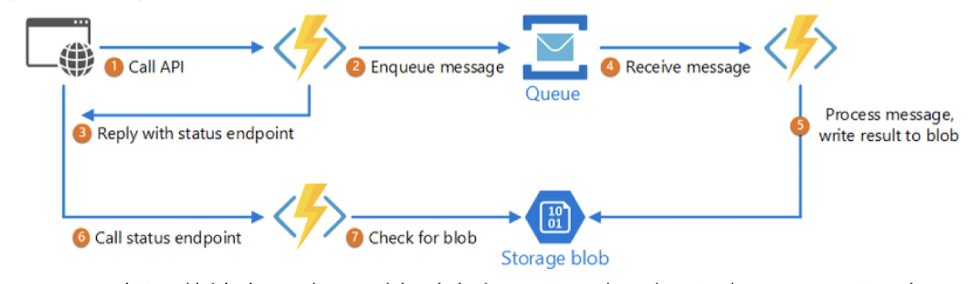
\includegraphics[width=0.85\linewidth]{4_async_request_reply.png}
    \end{itemize}

    \subsection{Event VS Message}
    \begin{itemize}
      \item \textbf{Similarities:} Both utilize async communication, facilitate decoupling of services, carry some info from 1 to other services to consume
      \item \textbf{Differences:}
      \begin{itemize}
        \item \underline{Event:} Carries an info which is a fact, a state change, something which has happened in the past $|$ Events are broadcasted for other services to consume \& typically use Pub-Sub pattern $|$ Publisher owns the event payload \& underlying channel (Topic) on which events gets published
        \item \underline{Message:} Carries a request (command/query) to be executed by another service $|$ Messages are point-to-point interactions between 2 services $|$ Receiver owns the message payload \& underlying channel (Queue) on which messages are published
      \end{itemize}
      \item \textbf{Topic VS Queue:}
      \begin{itemize}
        \item \underline{Topic:} Enables one-to-many communication, reaching multiple subscribers simultaneously $|$ Allows for non-sequential processing
        \item \underline{Queue:} Single receiver, ensuring each message reaches one receiver $|$ follows FIFO principle
      \end{itemize}
      \item \textbf{Design Examples}
      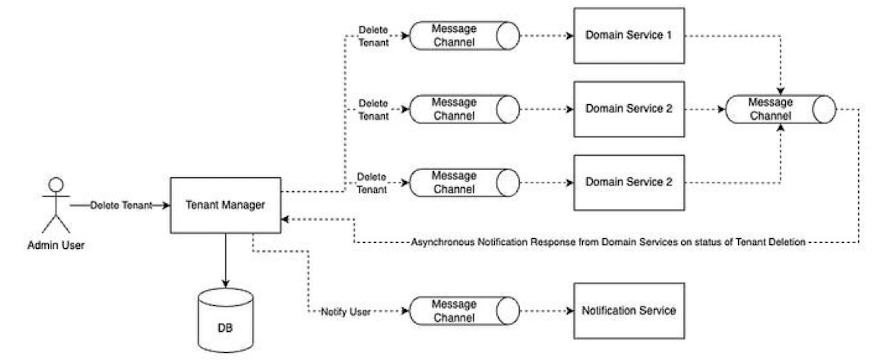
\includegraphics[width=0.85\linewidth]{5_design_example.png}
      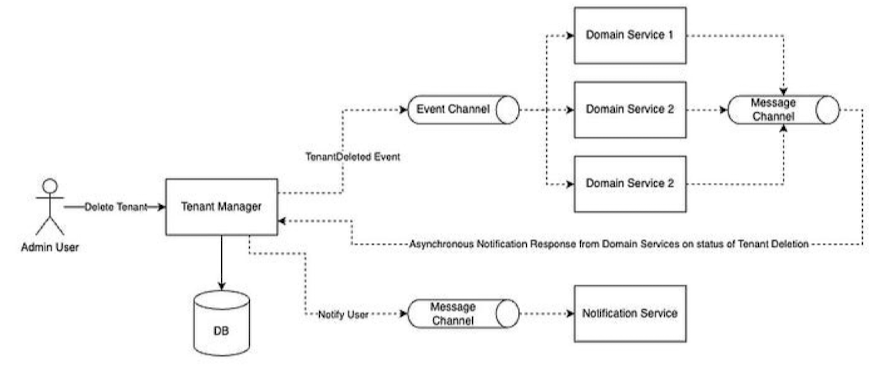
\includegraphics[width=0.85\linewidth]{6_design_example.png}
    \end{itemize}

    \subsection{Protocols \& Brokers}
    \begin{itemize}
      \item \textbf{Pub-Sub Broker (Multiple Receiver/Topic/Event-based)}
      \begin{itemize}
        \item Eg. Kafka $\rightarrow$ Each Kafka Broker is responsible for delivering the event to right consumer $|$ Can add as many brokers we need without any downtime (enables horizontal scaling)
        \item Unit of data within Kafka is an Event $\rightarrow$ Events are categorized into Topics $\rightarrow$ Topics are broken down into partitions $\rightarrow$ All events produced with given key get written to same partition
      \end{itemize}
      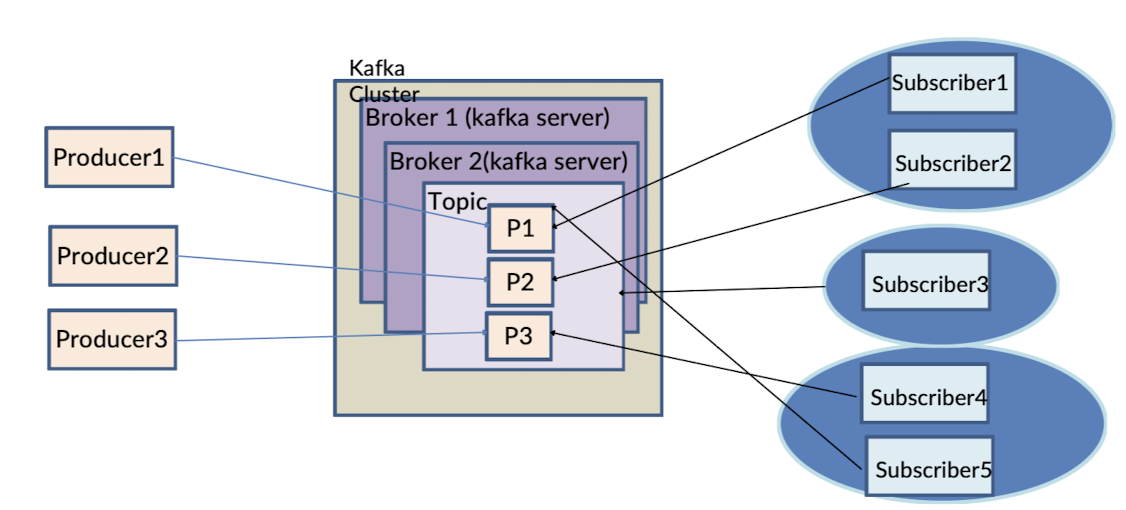
\includegraphics[width=0.7\linewidth]{7_kafka.png}
      \item \textbf{AMQP (Advanced Message Queuing Protocol) (Can both configured for both topic \& queue)}
      \begin{itemize}
        \item Messages are published to exchanges $\rightarrow$ Exchanges then distribute message copies to queues $\rightarrow$ Broker either deliver messages to consumers subscribed to queues OR Consumers pull messages from queues on demand
        \item Protocol can be used with any programming language (Can be used by any client that supports AMQP in any language)
        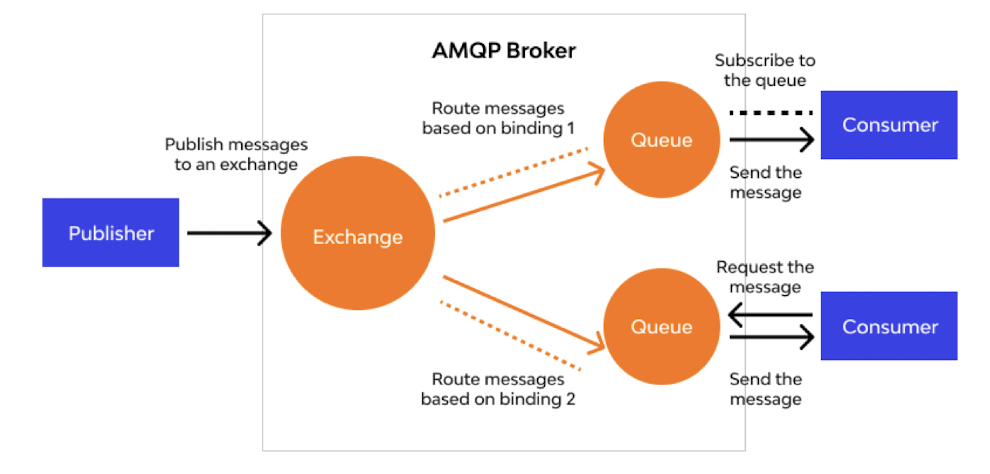
\includegraphics[width=0.75\linewidth]{8_AMQP_Broker.png}
        \item \underline{Exchange Types:} \\
        \textit{NOTE: Binding is a link set up to bind a queue to an exchange $|$ Routing key is message attribute the exchange looks at when deciding how to route the message to queues}
        \begin{enumerate}
          \item \textit{Direct:} Message is routed to queues whose binding keys exactly matches the routing key of the message (1-to-1)
          \item \textit{Fanout:} Fanout exchange routes messages to all queues bound to it (1-to-many)
          \item \textit{Topic:} Topic exchange does a wildcard match between routing key \& routing pattern specified in the binding (1-to-many)
        \end{enumerate}
      \end{itemize}
    \end{itemize}

    \subsection{Persistent VS Transient Communication}
    \begin{itemize}
      \item \textbf{Persistent Communication:} Messages are stored at each intermediate hop along the way until next node is ready to take delivery of message
      \item \textbf{Transient Communication:} Messages are buffered only for small periods of time $\rightarrow$ If message cannot be delivered or next host is down, message is discarded
    \end{itemize}

    \section{Messaging Patterns}
    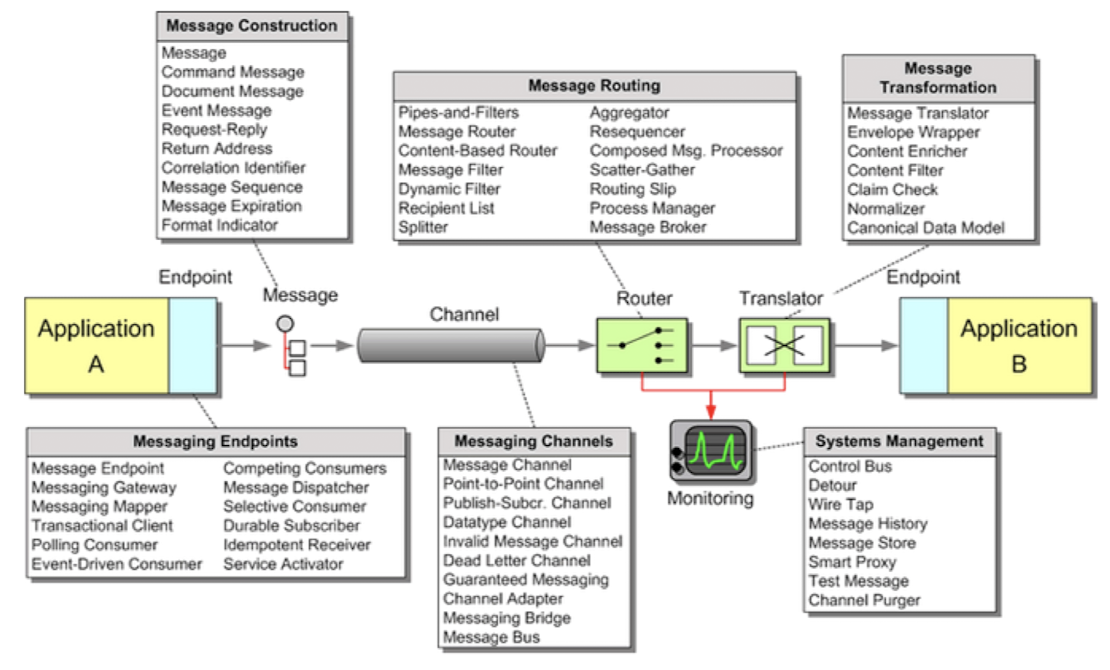
\includegraphics[width=0.85\linewidth]{9_Messaging_Patterns.png}

    \subsection{Message Construction}
    \begin{itemize}
      \item Message includes a header specifying type of info being transmitted, its origin, destination, size \& other structural info
      \item Message includes a payload containing actual info
      \item Message includes optional properties that are used for message selection \& filtering
    \end{itemize}

    \subsection{Message Channel}
    \begin{itemize}
      \item \textbf{One-way Property:} A channel transmits messages in 1 direction, 2-way message needs a 2-way channel (Eg. Request-and-reply each needs its own channel)
      \item \textbf{Return Address:} Request contains a return address to tell replier where to send reply to
      \item \textbf{Correlation ID:} Reply should contain Correlation ID that specifies which request this reply is for (Message ID of Request == Correlation ID of Reply, Correlation ID of initial Request will be null)
      \item \textbf{Special Purpose Channels:} \underline{Invalid Message Channel} (Handles erroneous messages) $|$ \underline{Dead Letter Channel} Handles message that could not be delivered $|$ \underline{Datatype Channel} (For specific type of data, all messages on a given channel contain same data type) 
      \item \textbf{Pub-sub Channels:} Used when multiple parties are interested in certain messages (Any message published to a topic is received by all topic subscribers) $\rightarrow$ Pub-sub request-response patterns are useful when it is important to communicate with multiple services that do parallel work, but their responses need to be aggregated afterwards \textit{(NOTE: Pub-sub channel for request messages, P2P channel for response messages)}
    \end{itemize}

    \subsection{Message Routing}
    \begin{itemize}
      \item \textbf{Message Routers:} Consume messages from 1 message channel \& reinsert them into different message channels, depending on a set of conditions
      \item \textbf{Simple Routers:} Route messages from 1 inbound channel to $\geq 1$ outbound channel
      \item \textbf{Composed Routers:} Combine multiple simple routers to create more complex message flows
      \item \textbf{Context-based Router:} Decides the message's destination based on specific contexts (used for load balancing, test or failover functionality)
      \item \textbf{Content-based Router:} Examines message content \& routes message onto a different channel based on message data $|$ has to have knowledge of all possible recipients \& their capabilities $|$ Changes in recipient list leads to change in content-based router
      \begin{itemize}
        \item \underline{Message Filter:} Special kind of Content-based router that eliminates undesired messages from a channel based on a set of criteria $|$ has only 1 output channel (for accepted message)
        \item \underline{Comparison against Pub-Sub Channel with Message Filter:} Content-Based Router has exactly 1 consumer receiving each message, Central control and maintenance, Needs to know about participants, Often used for business transactions like orders, Generally more efficient with queue-based channels $|$ Pub-Sub Channel with Message Filter can have $\geq 1$ consumer to consume a message, Distributed control and maintenance, No knowledge of participants required, Used for event notifications/info messages, Generally more efficient with Pub-Sub Channels
      \end{itemize}
      \item \textbf{Message Splitter:} A single message split into multiple messages $\rightarrow$ Each message can then be routed using a Content-Based Router
      \item \textbf{Message Aggregator:} Multiple messages aggregated into a single message $\rightarrow$ Aggregator then publishes message to output channel for processing
      \item \textbf{Message Scatter-Gather:} Routes/broadcasts single message to multiple participants concurrently \& reassembles/aggregates replies into single message $\rightarrow$ Ideal for requesting responses from multiple parties \& then aggregating and processing that data
      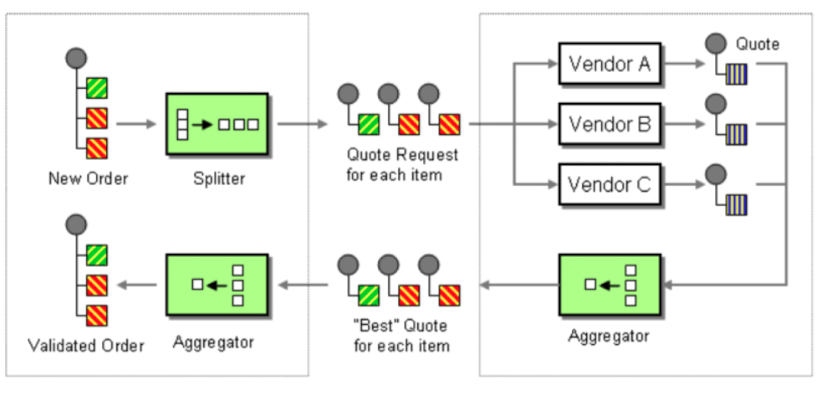
\includegraphics[width=0.85\linewidth]{10_splitter_agg_sg.png}
    \end{itemize}

    \subsection{Message Transformation}
    \begin{itemize}
      \item \textbf{Message Translator:} Converts messages from one format into another $\rightarrow$ resolves differences in message formats without changing the apps or having apps know about each other's data format, but if large number of apps communicate with each other, 1 Message Translator may be needed btw. each pair of communicating apps
      \item \textbf{Canonical Data Model:} Provides additional level of indirection btw. app's individual data formats $\rightarrow$ System A sends data to System B by first translating its data into canonical format, System B then receives data from System A and translates canonical format into its own data format
    \end{itemize}

    \subsection{Message Endpoint}
    \begin{itemize}
      \item \textbf{Definition:} Message Endpoint is interface btw. an app and a messaging system  $\rightarrow$ Used to send messages or receive them, but 1 instance does not do both $\rightarrow$ Endpoint is channel-specific (Single app will use multiple endpoints to interface with multiple channels)
      \item \textbf{Main Endpoint Types:} MessageProducer \& MessageConsumer
      \item \textbf{Consumer Endpoints:}
      \begin{enumerate}
        \item \underline{Polling Consumer:} Proactively reads messages once it is ready to consume them (Wants to control when it consumes each message)
        \item \underline{Event-Driven Consumer:} Reactively processes a message on its arrival (Message delivery is an event that triggers receiver into action)
      \end{enumerate}
    \end{itemize}
    
    \section{Object Interaction Design Patterns}
    \subsection{Design Pattern}
    \begin{itemize}
      \item \textbf{Definition:} Design Pattern is a solution \textit{(General design that can be applied to problems in this context)} to a problem \textit{(Goal to be achieved in the context)} in a context \textit{(Recurring situation in which pattern applies)}
      \item \textbf{Bridge Pattern:} Used to decouple an abstraction from its implementation via composition (not inheritance), so they can evolve independently $\rightarrow$ Useful when extending a class's functionality in multiple ways without creating a proliferation of subclasses
      \begin{itemize}
        \item Normally consists of (1): Abstraction, (2): Refined Abstraction, (3): Implementation, (4): Concrete Implementation, where Abstraction contains Implementation
      \end{itemize}
      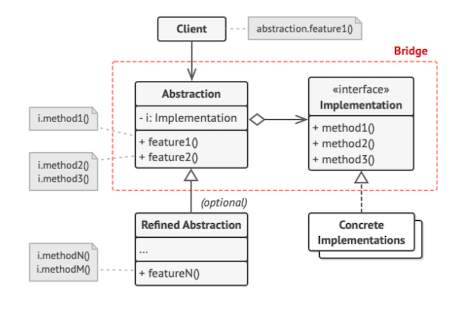
\includegraphics[width=0.7\linewidth]{11_bridge_pattern.png}
      \item \textbf{Proxy Pattern:} Use an intermediary object (Proxy) between a base object and its clients $\rightarrow$ Clients no longer have direct reference to base object, but instead interact with proxy $\rightarrow$ Proxy has reference to base object \& implements same interface as base object (Proxy contains base object)
    \end{itemize}
    
    \subsection{GoF Patterns}
    \begin{itemize}
      \item \textbf{Pattern Categories}
      \begin{enumerate}
        \item \underline{Creational:} Help designers handle object creation issues (Eg. Factory)
        \item \underline{Structural:} Provide a structure to relationship btw. objects (Eg. Facade, Bridge, Proxy, Adapter)
        \item \underline{Behavioral:} Define how objects interact with each other to deliver a task (Eg. Observer, Mediator)
      \end{enumerate}
      \item \textbf{Adapter Pattern:} Useful to reconcile differences btw. 2 incompatible interfaces, allowing them to work together seamlessly (Adapter is a class that implements the client interface, while wrapping the service object) \\ 
      (+): Single Responsibility Principle (Separate interface/data conversion code from primary business logic) $|$ Open/Closed Principle (Can introduce new types of adapters without breaking existing client code) \\
      (-): Increased code complexity due to new interfaces \& classes
      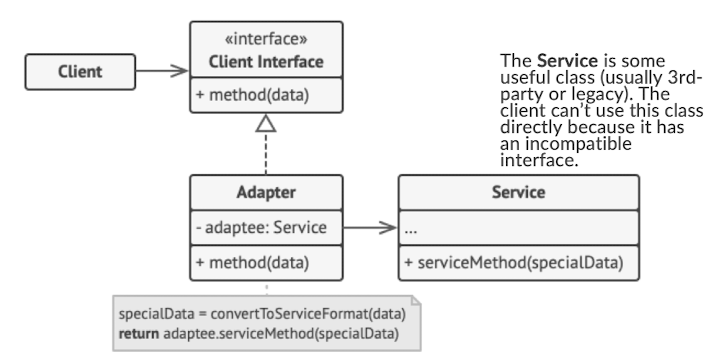
\includegraphics[width=0.8\linewidth]{12_adapter_pattern.png}
      \item \textbf{Facade Pattern:} Provide a unified interface to a set of interfaces in a subsystem $\rightarrow$ Clients interact with the facade instead of individual subsystem (Eg. API Gateway) \\
      (+): Isolate Code from complexity of subsystem $|$ (-): Facade can become god object coupled to all classes \\
      \textit{NOTE: Difference btw. Facade \& Adapter is that Facade focuses more on simplifying \& unifying access, while Adapter focuses more on improving compatibility (Eg. RCS Communicator component is more of an Adapter)}
      \item \textbf{Observer Pattern:}
      \begin{itemize}
        \item Defines a one-to-many dependency btw. objects so that when Observable changes state, all Observers are notified and updated
        \item Observers register themselves to Observable because they want to be notified when there is a change
        \item (+): Open/Closed Principle $|$ Can establish relations btw. objects at runtime $|$ (-): Observers are notified in random order
        \item \underline{Push Model:} Observable changes state $\rightarrow$ Notifies all observers $\rightarrow$ Observer calls back to Observable to retrieve more detailed info
        \item \underline{Pull Model:} Observable changes state $\rightarrow$ Subject pushes a snapshot of its state to all observers
      \end{itemize}
      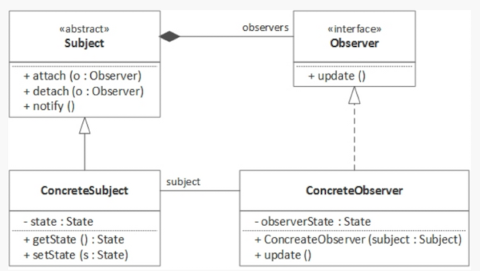
\includegraphics[width=0.65\linewidth]{13_observer_pattern.png}
      \item \textbf{Mediator Pattern:} Define an object that encapsulates how a set of objects interact $\rightarrow$ Promotes loose coupling by keeping objects from referring to each other explicitly \& letting us vary their interaction independently $\rightarrow$ If an object is updated with new interaction rules or a new object is added, only mediator object needs to be updated \\
      (+): Single Responsibility Principle (extract communication into single place) $|$ Open/Closed Principle $|$ Reduce coupling \& reuse components $|$ (-): Mediator can become god object
      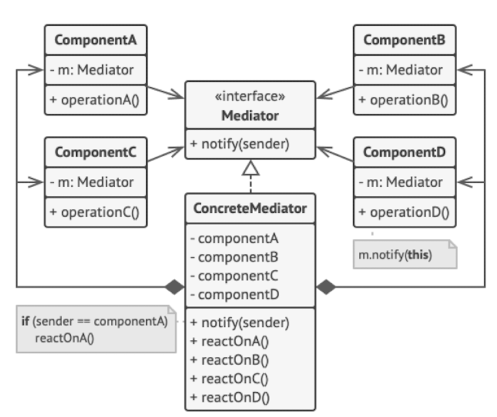
\includegraphics[width=0.65\linewidth]{14_mediator_pattern.png}
      \item \textbf{Data Transfer Object (DTO) Pattern:} A group of values in an ad-hoc structure just for purpose of passing data around (No business logic, only contain storage, accessors, serialization/parsing methods) $\rightarrow$ Reduces roundtrips to server by batching up multiple parameters in a single call
    \end{itemize}
\end{multicols*}
\end{document}
